\documentclass{article}
\usepackage[english]{babel}
\usepackage[utf8]{inputenc}
\usepackage{fancyhdr}
\usepackage{amsmath}
\usepackage{pdfpages}
\usepackage{graphicx}
\graphicspath{ {./images/} }

\pagestyle{fancy}
\fancyhf{}
\rhead{CS760}
\lhead{Cheng-Wei Lu}
\rfoot{Page \thepage}

\begin{document}

\section*{CS 760 Homework 3 by Cheng-Wei Lu}

\subsection*{Problem 3.1}
I normalize all non-nominal features and add an intercept to every data.

\subsubsection*{(a)}
	I set the iteration number of $\hat{\theta}$ update to 50000. Original step size = 1/20. I change the step size by multiply it with 3/4 every 50 iterations. The stop criteria is that when iteration number reaches 1000 or when the improvement for likelihood is less than $10^{-5}$, the parameter update will stop.

\subsubsection*{(b)}
	It took about 57 seconds for my computer to converge.
\subsubsection*{(c)}
	Please note that I have normalized all non-nominal features in my data.
	\begin{equation*}
		\hat{\theta} =  \begin{pmatrix} -4.097\text{(class )}\\  2.957\text{(sex)}\\ -2.070\text{(age)}\\ -0.259\text{(siblings/spouses aboard)}\\-0.033\text{(parents/children aboard)}\\ -0.038\text{(fare)}\\4.773\text{(intercept)} \end{pmatrix} 	
		\end{equation*}
	
\subsubsection*{(d)}
	likelihood $ = -399.89523993 $
	
\subsubsection*{(e)}
	The distribution of $\hat{\theta}$ is $N(\theta^*, I^{-1}_{\theta^{*}})$, where the $\theta^*$ is the real $\theta$ and the variance is represented by a covariance matrix $I^{-1}_{\theta^{*}}$, which is of the following  value :
	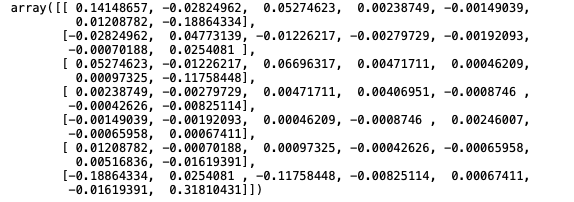
\includegraphics[scale=0.5]{fisher_v2}
	
\subsection*{Problem 3.2}
\subsubsection*{(a)}
	By the invariance property of MLE, we know that  $\hat{w} = x^T\hat{\theta}$.
\subsubsection*{(b)}
	Since  $\hat{\theta}  \xrightarrow[]{d} N(\theta^*, I^{-1}_{\theta^{*}})$, and $\hat{w} = x^T\hat{\theta}$. It implies  $\hat{w}  \xrightarrow[]{d} N(x^{T}\theta^*, x^{T}I^{-1}_{\theta^{*}}x)$.

\subsection*{Problem 3.3}
	For this part, I create a data as follow:
	\begin{equation*}
		x=  \begin{pmatrix} 2 \text{(class)}\\ 0 \text{(sex)}\\ 25\text{(age)}\\ 0\text{(siblings/spouses aboard)}\\0\text{(parents/children aboard)}\\ 50\text{(fare)}\\1\text{(intercept)} \end{pmatrix} 	\end{equation*}
	Therefore, the normalized data would be :
	\begin{equation*}
		x_{normalized} =  \begin{pmatrix} 0.867 \text{(class)}\\ 0 \text{(sex)}\\ 0.848\text{(age)}\\ 0\text{(siblings/spouses aboard)}\\0\text{(parents/children aboard)}\\ 1.547\text{(fare)}\\1\text{(intercept)} \end{pmatrix} 	\end{equation*}

\subsubsection*{(a)}
	According to the logistic prediction and setting odds threshold bigger than 1/2 as being able to survive,  I would not have survived the sinking because that I am a male and I am not young and rich enough. Just like in the movie - they have to let women and children escape first.
	
\subsubsection*{(b)}
	According to the prediction,the log odds would be $-0.5965$ . The variance for odds is calculated according to $x^{T}I^{-1}_{\theta^{*}}x$. The standard deviation is therefore $0.1444$. The z value for $\alpha = 0.05$ is approximately 1.96, therefore the confidence interval for my log odds of survival is $[-0.8797, -0.3133 ]$.
	
\subsubsection*{(c)}
	If we are talking about the odds, I think has big variance. But if we are talking about whether I would have died, it is certain because with 95 percent confidence, even the at upper bound of my odds interval, my probability to have survived is 0.422, which  is still  less than 1/2 ( the standard to see if one would have died).
	
\subsection*{Problem 3.4}
\subsubsection*{(a)}
	
	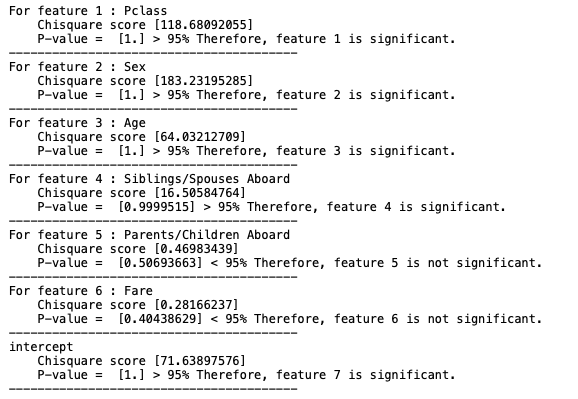
\includegraphics[scale=0.5]{test_v2}
	I used $\frac{\hat{\theta}^{2}_{J}}{v_j^{2}}$ to calculate the chi-score for each feature, and
	
\subsubsection*{(b)}
	Based on the result above, pclass ,sex, age, siblings/spouses aboard, and intercept are significant features.
	
\subsubsection*{(c)}
	The most significant feature is sex according to the chi-square score. If I change my sex, I would be alive with the probability of survival  equal 0.913.	
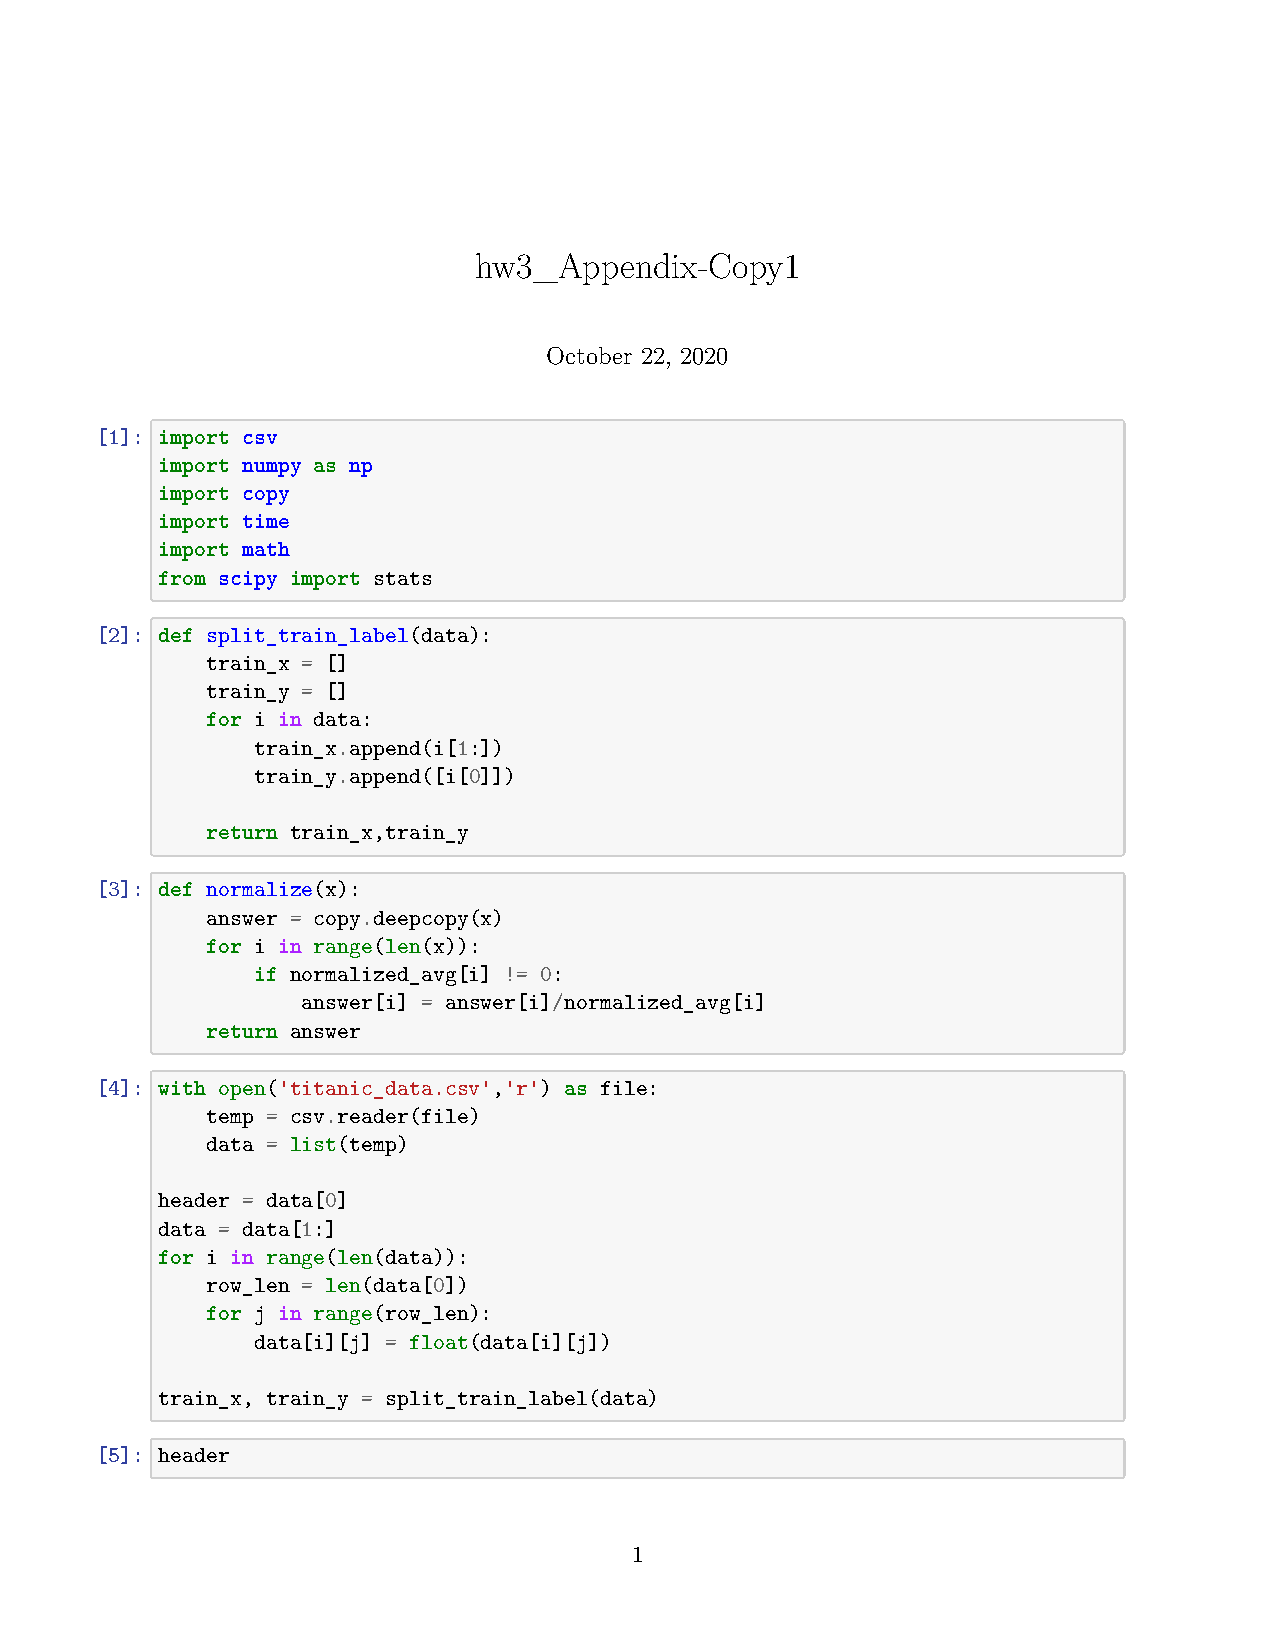
\includepdf[page={1,2,3,4,5,6}]{hw3_Appendix-Copy1.pdf}
\end{document}

